\section{Background}
\label{sec: background}
In this section, we introduce the database systems used in our evaluation (Section~\ref{subsec: evaluated-systems}), and we present the key features of the PPS workload that represent the foundation of our benchmarking framework (Section~\ref{subsec: product-parts-supplier-workload}).

\subsection{Evaluated Systems}
\label{subsec: evaluated-systems}
This study evaluates four database systems that support globally distributed transactions: Calvin, SLOG, Detock, and Janus, using the benchmarking framework we implemented. Each system has its unique deployment strategy and concurrency control approach for handling distributed transactions.

We selected these four systems because they all support geo-distributed transactions and share comparable architectural principles, such as deterministic execution and graph-based serialization, which aim to reduce the runtime wide-area communication. Despite these foundational similarities, they have clear differences that make each system more suitable for particular workload characteristics or deployment scenarios. Another important aspect is that the Detock codebase\footnote{\url{https://github.com/umd-dslam/Detock}} provides a unified implementation of all four systems. So, Calvin, SLOG, and Janus were re-implemented within the Detock framework to share a common storage engine, communication layer, and local consensus protocol \cite{nguyen2023detock}. This shared infrastructure ensures that the performance differences from our evaluation come from each system's core design choices rather than unrelated implementation details.

\paragraph{Deterministic Scheduling.}
Calvin, SLOG, and Detock are based on \textit{deterministic scheduling}, an alternative to traditional protocols that use atomic commitment \cite{thomson2010case}. These deterministic database systems avoid the need for runtime coordination between different servers by predefining the execution order of the transactions. This design reduces the communication overhead during transaction execution, which offers notable performance benefits, especially in the presence of inter-region delays. However, this type of locking protocol requires complete knowledge of each transaction's read and write sets in advance. As a result, these systems face challenges when handling \textit{dependent transactions}, namely transactions for which the accessed records are not known beforehand, but must be discovered as the execution progresses.

\textit{Calvin}~\cite{thomson2012calvin} demonstrated the practical feasibility of deterministic transaction processing with near-linear scalability. The system is organized into three separate layers. First, the \textit{sequencing layer} receives the transactional requests from the clients, batches them using short epochs, and ensures consistent ordering among the replicas. Then, the \textit{scheduling layer} coordinates the transaction execution by acquiring the locks deterministically according to the defined global order and by passing the transactions to the pool of workers. Finally, the \textit{storage layer} handles the physical data access.

\textit{SLOG}~\cite{ren2019slog} is built on top of Calvin by optimizing for data locality when used in geo-distributed settings. It introduced the notion of \textit{single-home (SH) transactions} that access data in a single region, and thus can be processed with very low latency without being passed to the sequencing layer. However, the \textit{multi-home (MH) transactions} still follow Calvin's sequencing model and must adhere to a global order.

\textit{Detock}~\cite{nguyen2023detock} is also based on Calvin's architecture, but it removes the need for global ordering by using a deadlock resolution protocol via a \textit{dependency graph}. This approach allows both single-home and multi-home transactions to be scheduled deterministically at each region. In this way, all participating regions construct independently the same dependency graph, and the transactions can be run locally without the need for cross-region communication once all transaction components have been received.

\paragraph{Unified Consensus and Concurrency Control.}
\textit{Janus}~\cite{mu2016consolidating} integrates the concurrency control mechanism (used for transaction consistency) with the consensus protocol (used for replication) into a single layer. The key idea is that both components work by ensuring that the execution history of the transactions is equivalent to a sequential order, which can be verified by defining a \textit{serialization graph}. Janus can commit and replicate the transactions within a wide-area network round-trip under low contention, and requires at most one additional round-trip in case of conflicts.

\subsection{Product-Parts-Supplier Workload}
\label{subsec: product-parts-supplier-workload}
The Product-Parts-Supplier (PPS) workload is a well-known relational structure that simulates a realistic supply chain management system. It captures the interactions between the existing products, the parts that make up those products, and the suppliers that provide those parts.

PPS has been used as a workload in several popular database benchmarking studies, although typically in a limited capacity. For example, Harding et al.~\cite{harding2017evaluation} utilized the PPS workload primarily to evaluate the system scalability by varying only the number of client machines, while keeping the other settings fixed. Serafini et al.~\cite{serafini2016clay} applied the PPS in their evaluation, but they included only read-only transactions since their goal was to assess the effectiveness of their dynamic partitioning scheme rather than to evaluate the full concurrency behavior of the system.

Our benchmarking framework is built upon a set of tables and transaction types drawn from these previous uses of the PPS workload. Specifically, the schema includes three core entities, \textit{Products}, \textit{Parts}, and \textit{Suppliers}, along with two tables that capture their many-to-many relationships. A product can contain multiple parts, and a part can belong to multiple products. In the same way, a supplier can provide multiple parts, and a part can be provided by multiple suppliers. Figure~\ref{fig: pps-erd} shows the relational schema of the PPS workload.

\begin{figure}[ht]
    \centering
    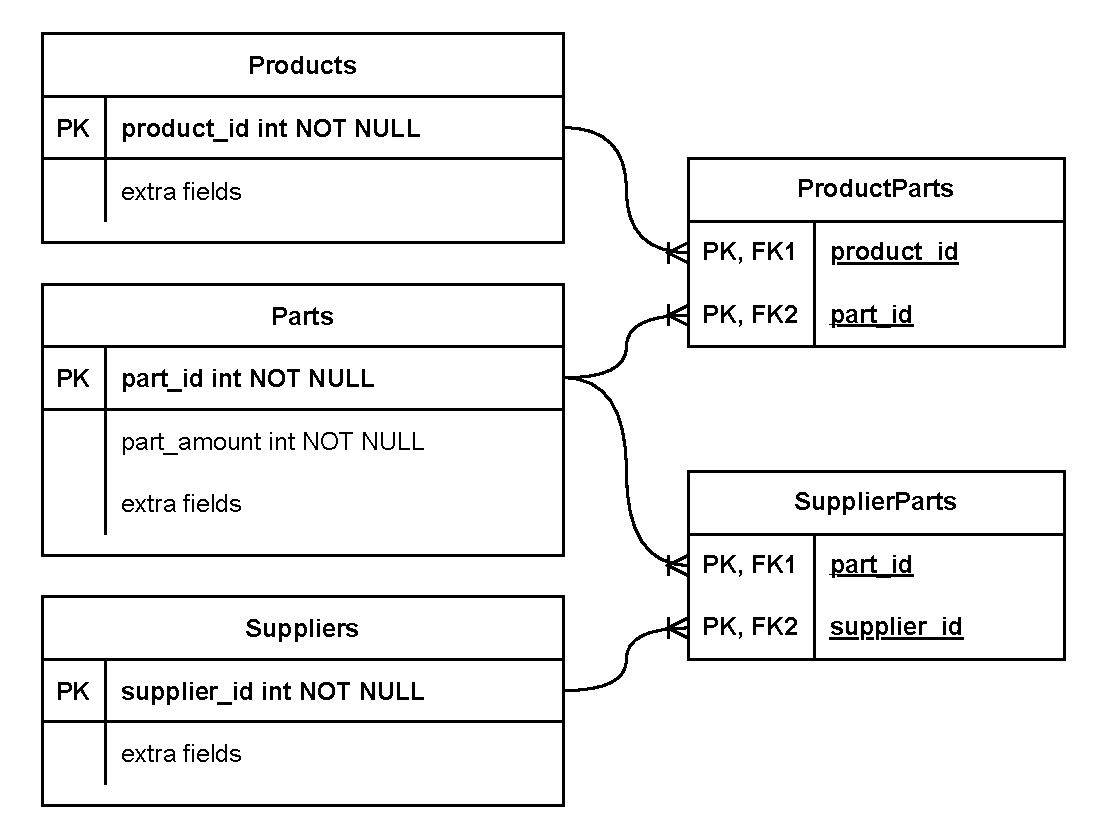
\includegraphics[width=1\linewidth]{figures/PPS ERD.pdf}
    \caption{Product-Parts-Supplier Entity Relationship Diagram.}
    \label{fig: pps-erd}
\end{figure}

The PPS workload has transactions with complex data dependencies that can lead to contention challenges when multiple transactions run concurrently. This complexity makes the workload suitable for evaluating how database systems handle the coordination and conflict resolution. The workload includes several types of transactions, namely:
\begin{itemize}
    \item \textit{OrderProduct}. Given a \texttt{product\_id}, this transaction will first collect the parts associated with the given product and then decrement the inventory amount for those parts. Importantly, this is a dependent transaction, since we do not know which parts will be updated in advance.
    \item \textit{GetPartsByProduct}. Given a \texttt{product\_id}, this transaction will retrieve the list of parts that are currently associated with the given product.
    \item \textit{UpdateProductPart}. Given \texttt{product\_id}, \texttt{part\_from}, and \texttt{part\_to}, this transaction will update a part associated with the given product by replacing the part identified with \texttt{part\_from} with the latter part \texttt{part\_to}.
    \item \textit{GetPart}. Given a \texttt{part\_id}, this transaction will retrieve the current inventory amount of the given part, along with any existing extra information.
    \item \textit{GetProduct}. Given a \texttt{product\_id}, this transaction will retrieve any extra information about the given product.
\end{itemize}